%!TEX root = proj_report_outline.tex
\appendix
\chapter{User Stories}\label{A:user_stories}

\begin{verbatim}

Feature: posting Pitch Card
  As a user, I want to create a Pitch Card so that the community and I may
  collaborate to find a solution

  Background:
    Given following users exist:
      | username    | email             |
      | Foo	        | foo@foo.foo       |
      | Bar      	| bar@bar.bar       |
      | Baz      	| baz@baz.baz       |
      | Qux      	| qux@qux.qux       |
    And I sign in as "foo@foo.foo"
    And I go to the new pitch card page

  Scenario: post well formed pitch card with seek and deselect
    When I specify the following pitch points:
      | value	        | Energy-saving agriculture innovation       |
      | opportunity     | High energy costs involved in running
       agriculture business could be decreased       |
      | solution        | A cost-effective innovation that uses
       renewable energy in the agriculture industry  |
    And I seek the following pitch points:
      | resources       |
      | facilitation    |
    And I deselect the following pitch points:
      | voting          |
    And I submit the pitch card
    Then I should see "Success"

   Scenario: post bogus Pitch Card
   ...

\end{verbatim}

\begin{verbatim}

Feature: viewing Pitch Cards dashboard
  As a user, I want to view the latest Pitch Cards added so that I may browse
  for Pitch Cards to contribute to

  Scenario: view dashboard
  ...

Feature: viewing my collaborated Pitch Cards
  As a user, I want to view Pitch Cards I have collaborated on so that I 
  may check on their progress

  Scenario: view collaborated
  ...

Feature: viewing my initiated Pitch Cards dashboard
  As a user, I want to view Pitch Cards I have initiated on so that I 
  may check on their progress

  Scenario: view intiated
  ...

Feature: search for Pitch Cards
  As a user, I want to search for Pitch Cards using keywords so that I may find
  Pitch Cards that I am interested in

  Scenario: search for "apples"
  ...

\end{verbatim}

\begin{verbatim}

Feature: annotate Pitch Point
  As a user, I want to suggest changes on viewable Pitch Cards so that I can offer insight

  Scenario: make a suggestions
  ...

  Scenario: delete a suggestion
  ...

  Scenario: make a comment
  ...

  Scenario: delete a comment
  ...

\end{verbatim}

\begin{verbatim}

Feature: scope pitch point suggestions
  As a user, I want to negotiate the scope of disclosure with the initiator for
   the content of my suggestion so that I may protect my IP's 
   dissemination

  Scenario: scope using public
  ...

  Scenario: scope using members
  ...

  Scenario: scope using contributors
  ...

  Scenario: scope using private
  ...

Feature: scope pitch point comments
  As a user, I want to negotiate the scope of disclosure with the initiator for
   the content of my comments so that I may protect my IP's 
   dissemination

  Scenario: scope using public
  ...

  Scenario: scope using members
  ...

  Scenario: scope using contributors
  ...

  Scenario: scope using private
  ...

\end{verbatim}

\begin{verbatim}

Feature: scope Pitch Cards
  As an initiator, I want to control the scope of disclosure of my Pitch Cards 
  so that I may protect my IP's dissemination

  Scenario: scope using public
  ...

  Scenario: scope using members
  ...

  Scenario: scope using private
  ...

\end{verbatim}

\begin{verbatim}

Feature: audit Pitch Card viewers
  As an initiator, I want to see who has viewed my content 

  Scenario: scope using public
  ...

  Scenario: scope using members
  ...

  Scenario: scope using private
  ...

\end{verbatim}

\begin{verbatim}

Feature: new user registration
  As an unregistered user, I want to join so that I may collaborate with the community

  Scenario: new user goes through the setup wizard
  ...

  Scenario: new user tries to use XSS
  ...

  Scenario: user fills in bogus data - client side validation
  ...

Feature: user authentication
  As a user, I want to log in so that I can interact with the system.

  Scenario: user logs in
  ...

  Scenario: user attempts to log in with bogus credentials
  ...

Feature: log out
  As a user, I want to log out so that I can keep my account safe

  Scenario: user logs out
  ...

Feature: reset password
  As a user, I want to reset my password in case I forget it

  Scenario: Reset my password
  ...

  Scenario: Attempt to reset password with invalid password
  ...
  
  Scenario: Attempt to reset password with invalid email
  ...

\end{verbatim}

\chapter{Content Template - Pitch Card}\label{A:content_template}

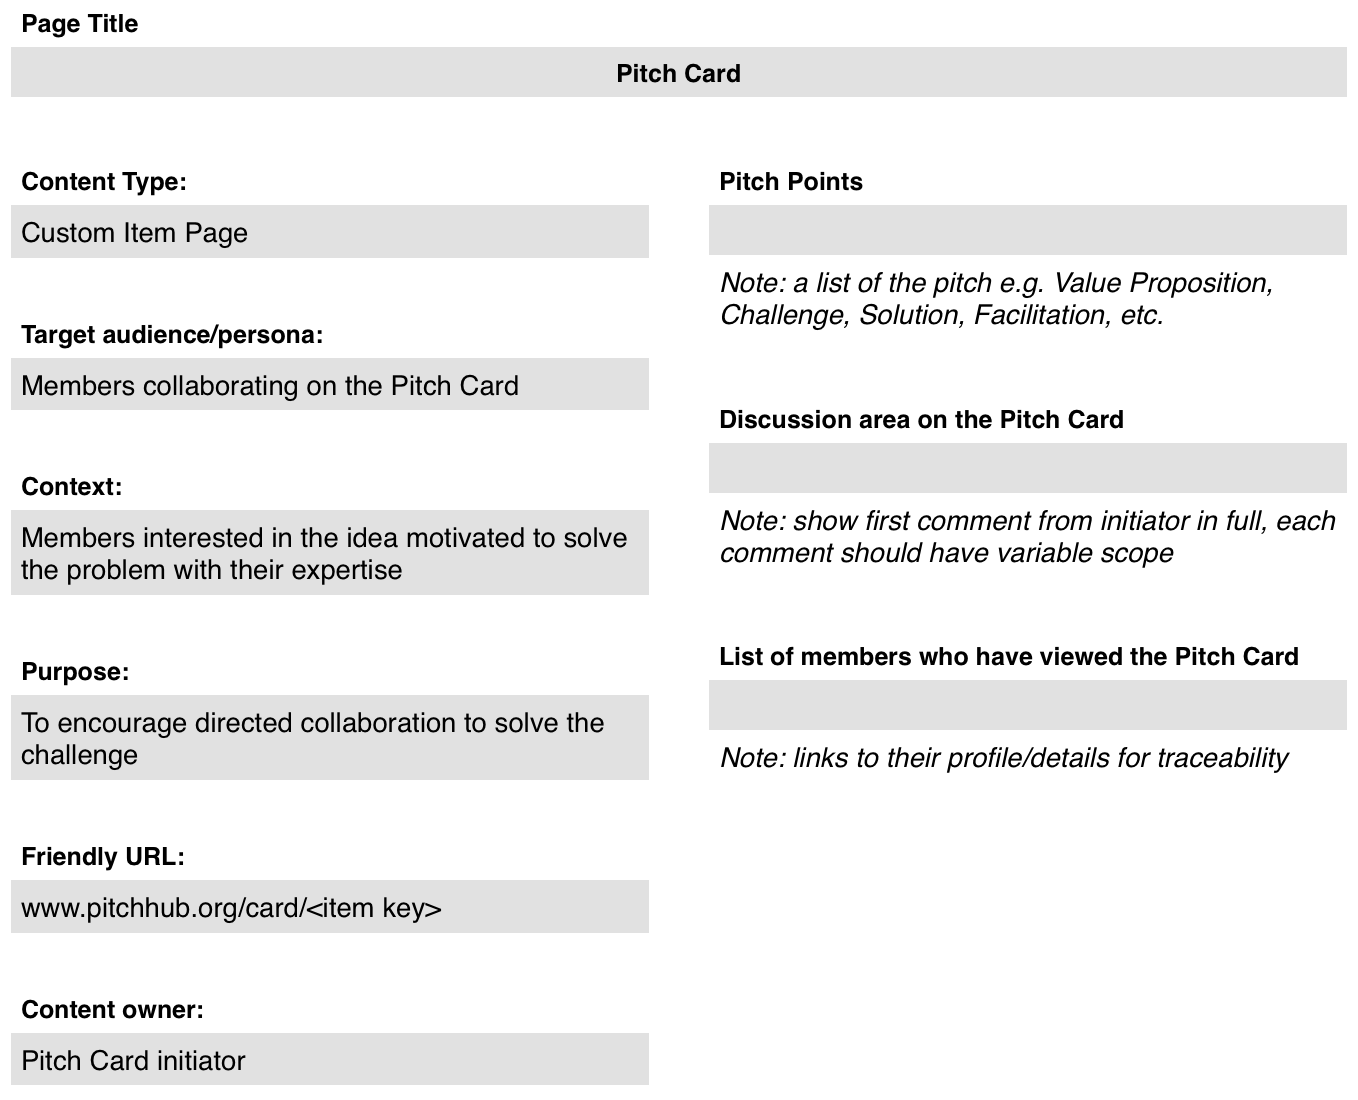
\includegraphics[width=1\textwidth]{show_pitch_card_content_template}

\chapter{Pitch Card Page Screenshot}\label{A:pitch_card_pitchhub}

\begin{sidewaysfigure}[ht]
    \centering
    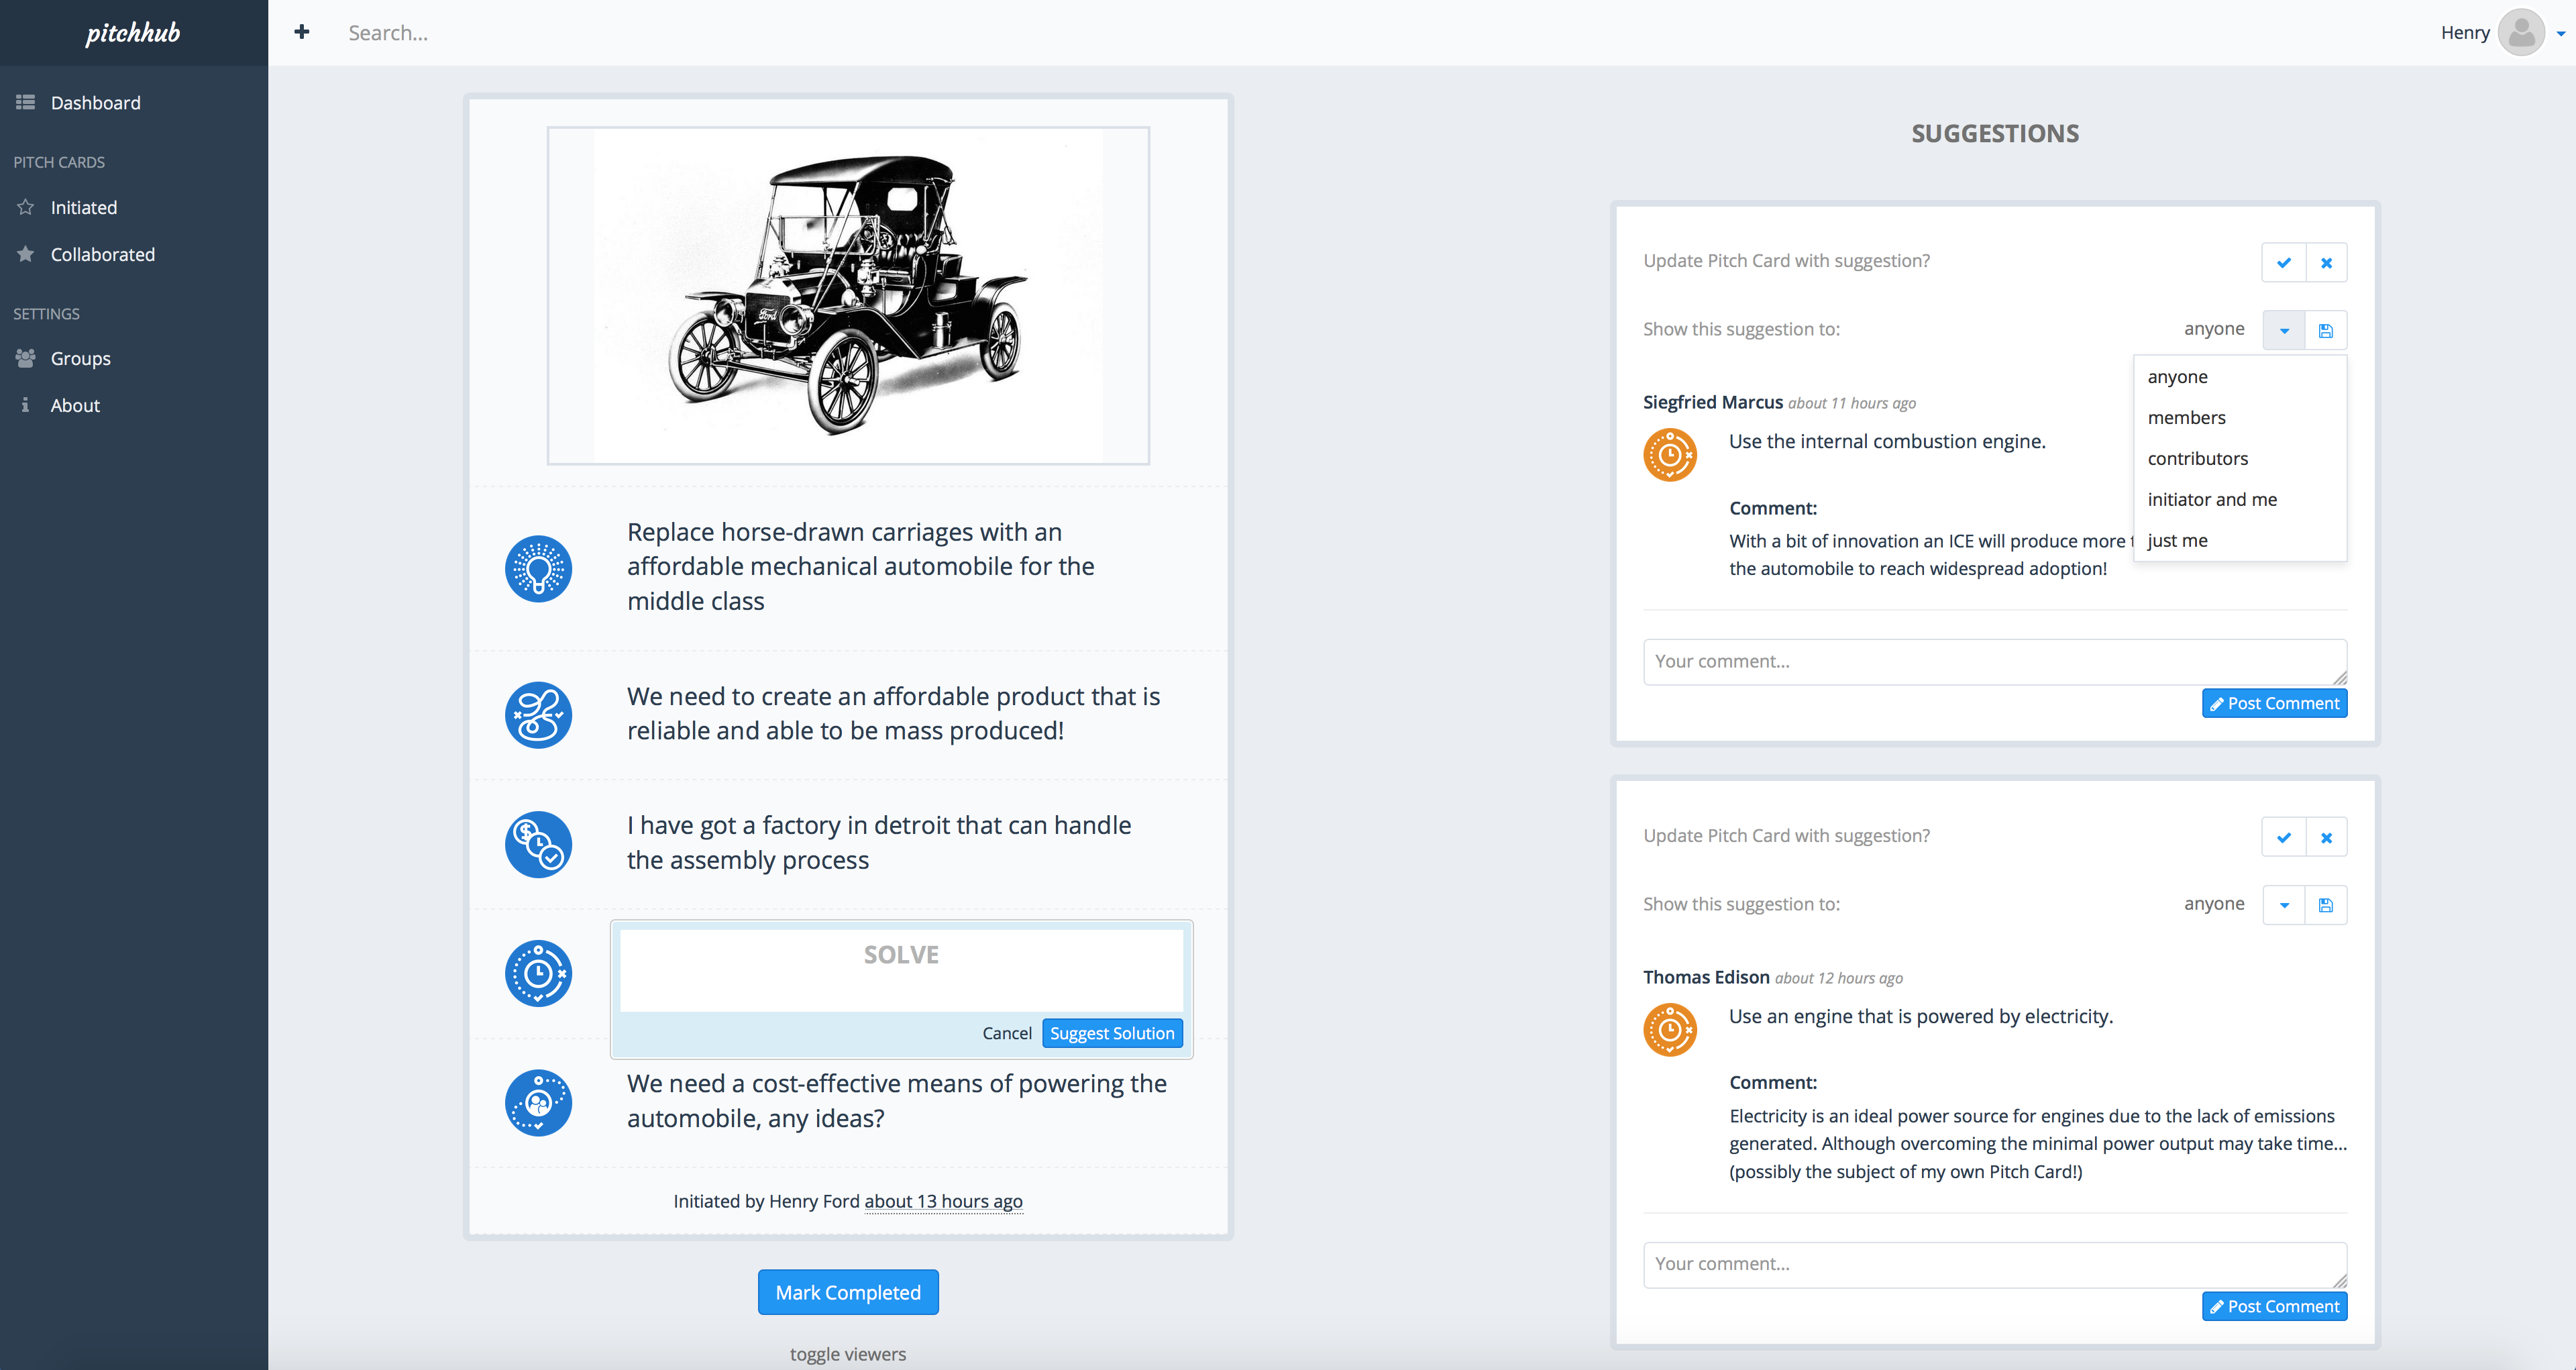
\includegraphics[width=1\textwidth]{pitch_card_view}
\end{sidewaysfigure}

\chapter{Dashboard Page Screenshot}\label{A:dashboard_pitchhub}

\begin{sidewaysfigure}[ht]
    \centering
    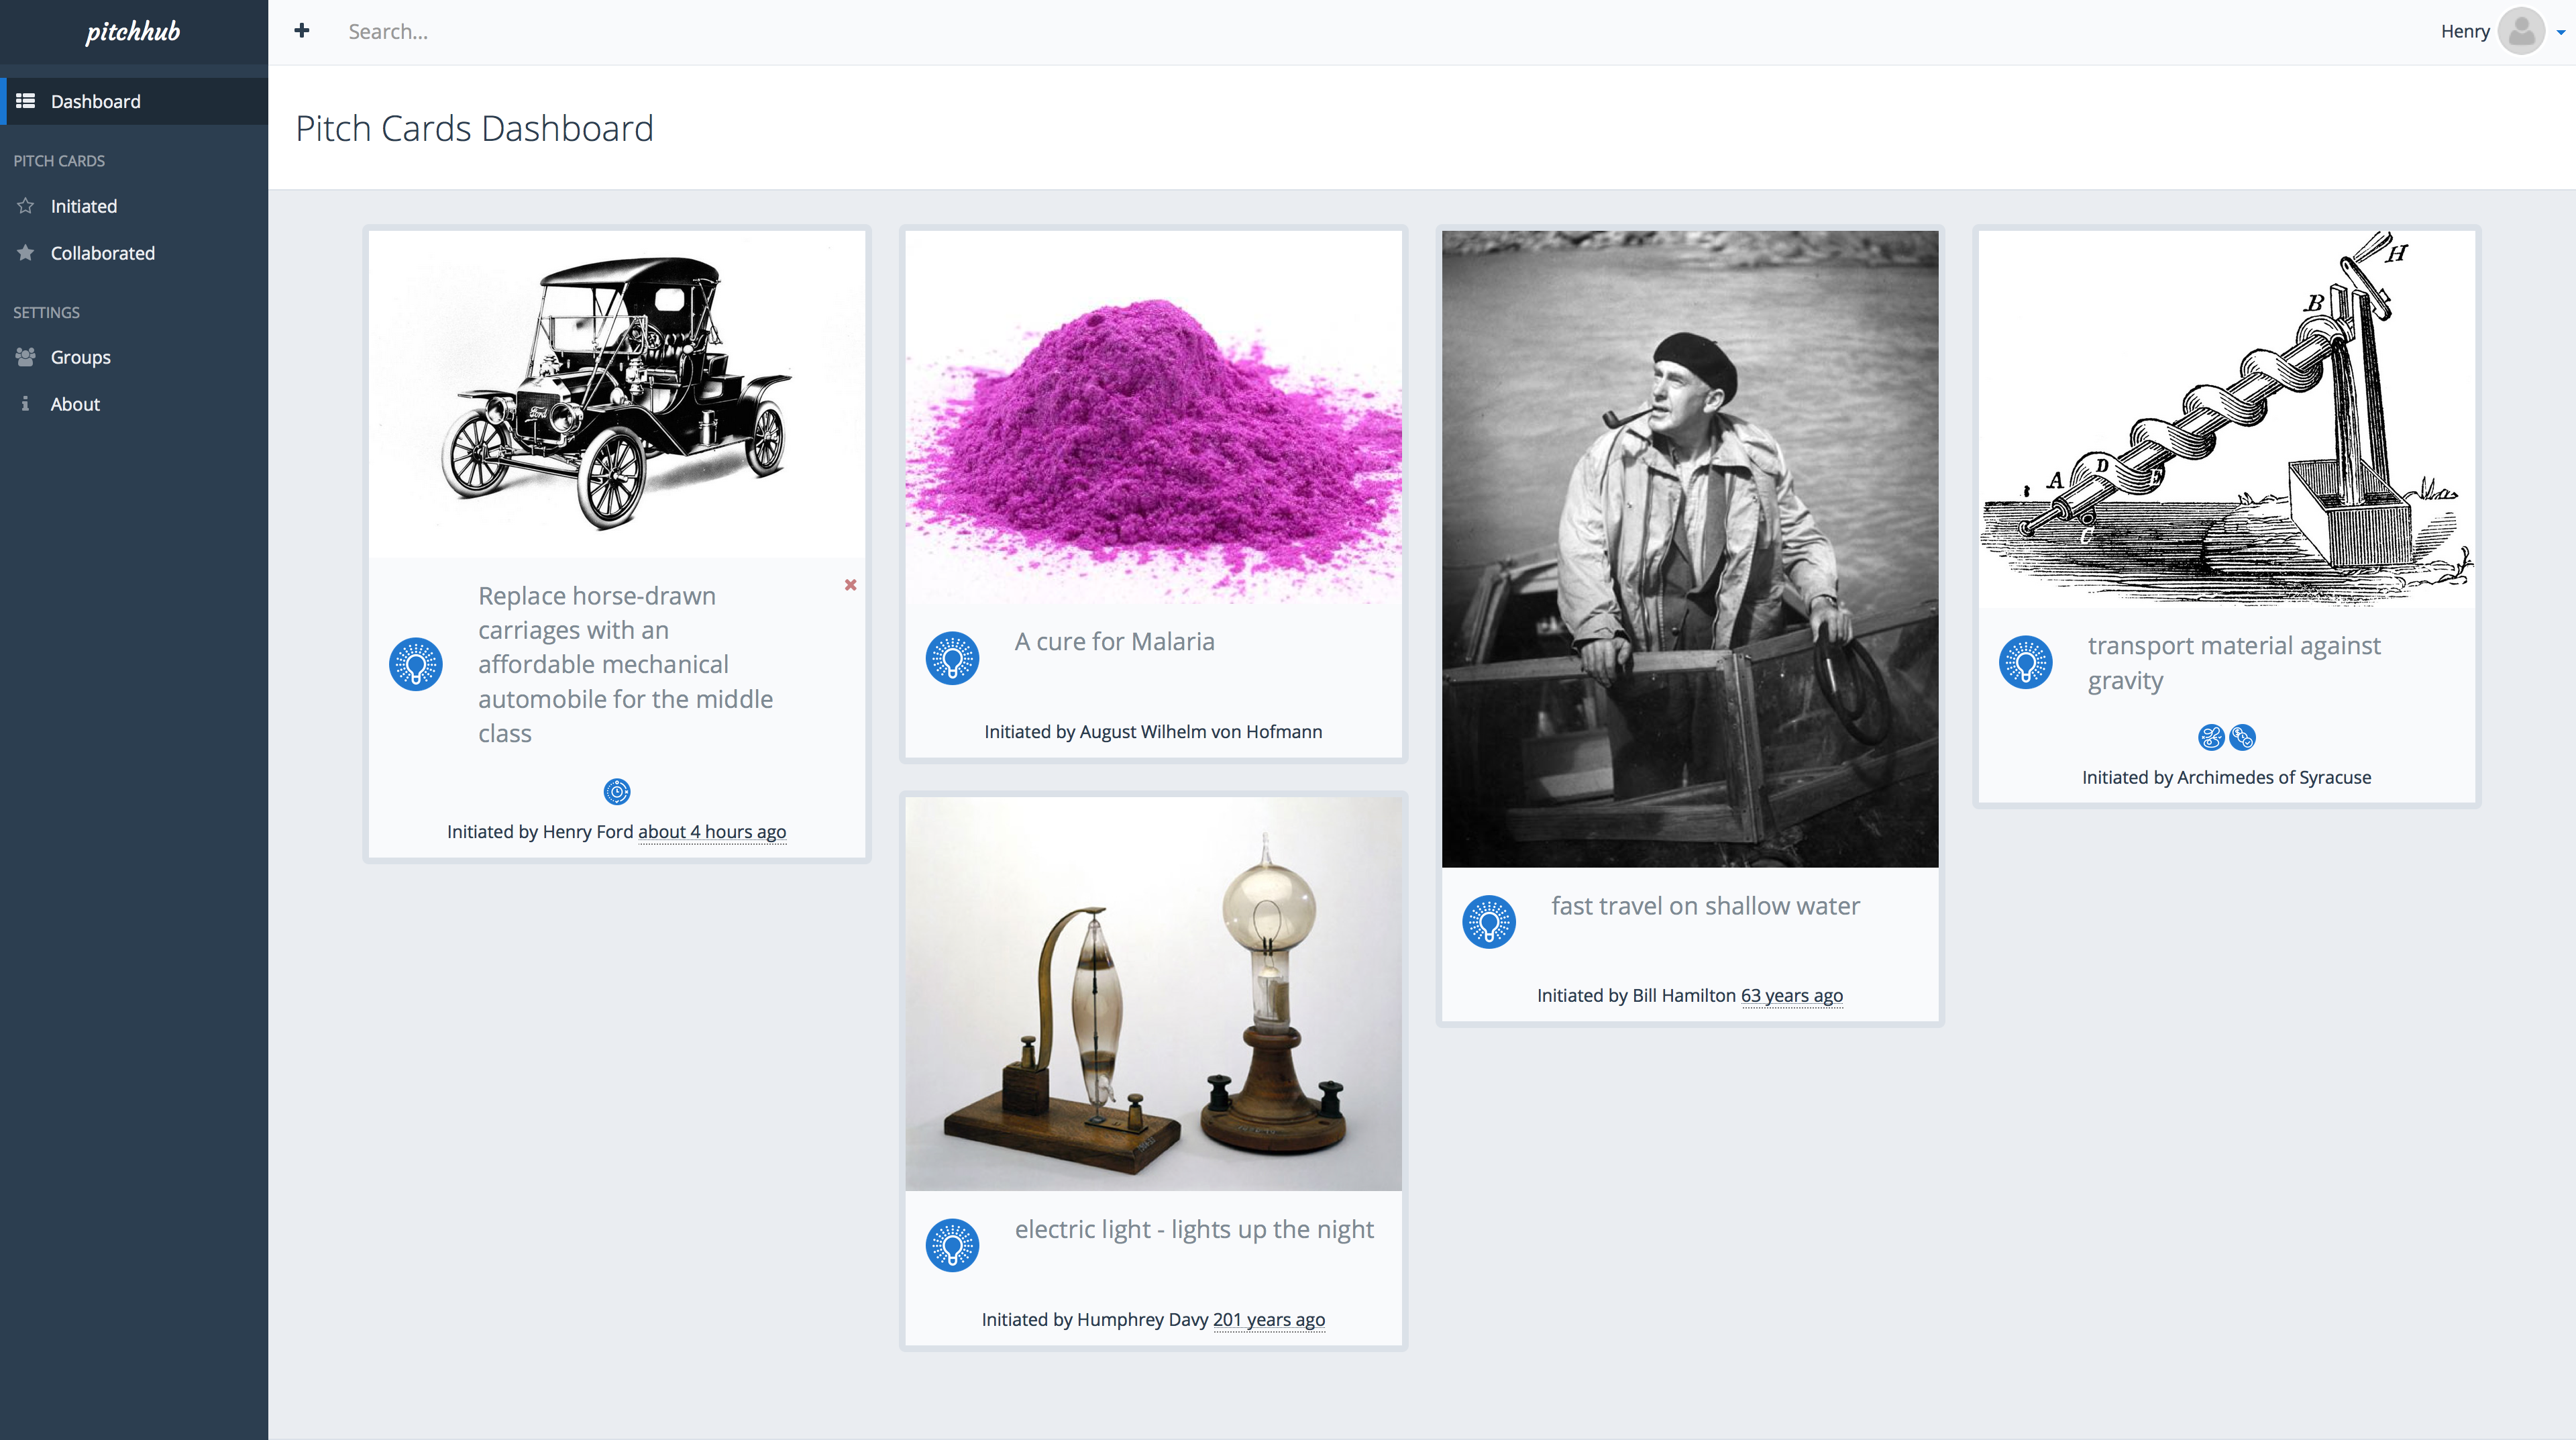
\includegraphics[width=1\textwidth]{dashboard_pitchhub}
\end{sidewaysfigure}

